% Diagrama de proveniência experimental formal — do dataset de origem ao artefato de relatório.
% Cadeia central simplificada, mas genuína: cada nó e relação usa exatamente os tipos
% PROV-O emitidos por src/coinfosim/provenance/model.py (build_scenario_prov_document),
% conforme docs/semantics/provenance_mapping.md e o grafo real regenerado de um cenário
% de escala completa (provenance.provn). Omite deliberadamente a atividade opcional de
% recuperação histórica de artefatos (coinfosim:ArtifactRecovery/RecoveredArtifactSet) e
% a entidade coinfosim:CodeRevision: são metadados de regeneração de relatório, não parte
% da proveniência científica do experimento (Real → Real / Gaussiana única → Real /
% GMM → Real), que é o objeto desta figura. Compilação: xelatex (determinística).
\documentclass[tikz,border=6pt]{standalone}
% Preâmbulo compartilhado dos diagramas conceituais do relatório CoInfoSim.
% Compilação: xelatex (determinística; nenhum dado experimental é usado).
\usepackage{fontspec}
\setmainfont{Liberation Sans}
\setsansfont{Liberation Sans}
\usepackage{amsmath}
\usepackage{bm}
\usepackage{tikz}
\usetikzlibrary{arrows.meta,positioning,calc,fit,backgrounds,decorations.pathreplacing,matrix,patterns}
\definecolor{CoinAccent}{RGB}{25,80,140}
\definecolor{CoinAccentDark}{RGB}{18,55,95}
\definecolor{CoinAccentPale}{RGB}{237,242,248}
\definecolor{CoinGray}{RGB}{95,95,95}
\definecolor{CoinGrayPale}{RGB}{246,246,246}
\definecolor{CoinWin}{RGB}{76,140,90}    % verde discreto (vitória)
\definecolor{CoinLose}{RGB}{182,88,79}   % vermelho discreto (derrota)
\tikzset{
  bloco/.style={draw=CoinAccentDark, fill=CoinAccentPale, rounded corners=1.2pt,
                align=center, font=\small, inner sep=4pt, minimum height=7mm},
  bloconeutro/.style={draw=CoinGray, fill=CoinGrayPale, rounded corners=1.2pt,
                align=center, font=\small, inner sep=4pt, minimum height=7mm},
  blocoreal/.style={draw=CoinAccentDark, fill=white, rounded corners=1.2pt,
                align=center, font=\small, inner sep=4pt, minimum height=7mm},
  seta/.style={-{Stealth[length=2.4mm]}, thick, CoinAccentDark},
  setacinza/.style={-{Stealth[length=2.4mm]}, thick, CoinGray},
  rotulo/.style={font=\footnotesize\itshape, text=CoinGray, align=center},
}


\definecolor{ProvEntity}{RGB}{250,232,168}
\definecolor{ProvEntityBorder}{RGB}{176,141,42}
\definecolor{ProvActivity}{RGB}{188,206,235}
\definecolor{ProvActivityBorder}{RGB}{47,86,145}
\definecolor{ProvAgent}{RGB}{244,206,178}
\definecolor{ProvAgentBorder}{RGB}{176,94,42}

\tikzset{
  entidade/.style={draw=ProvEntityBorder, fill=ProvEntity, rounded corners=6pt,
                align=center, font=\scriptsize, inner sep=4pt, minimum height=8.5mm, minimum width=3.65cm},
  atividade/.style={draw=ProvActivityBorder, fill=ProvActivity, rounded corners=1pt,
                align=center, font=\scriptsize, inner sep=4pt, minimum height=8.5mm, minimum width=3.65cm},
  agente/.style={draw=ProvAgentBorder, fill=ProvAgent, rounded corners=1pt,
                align=center, font=\scriptsize, inner sep=4pt, minimum height=8mm, minimum width=3.0cm},
  relacao/.style={-{Stealth[length=2.0mm]}, thick, CoinGray},
  relacaofina/.style={-{Stealth[length=1.8mm]}, thin, CoinGray},
  rlabel/.style={font=\tiny\itshape, text=CoinGray, fill=white, inner sep=1pt},
}

\begin{document}
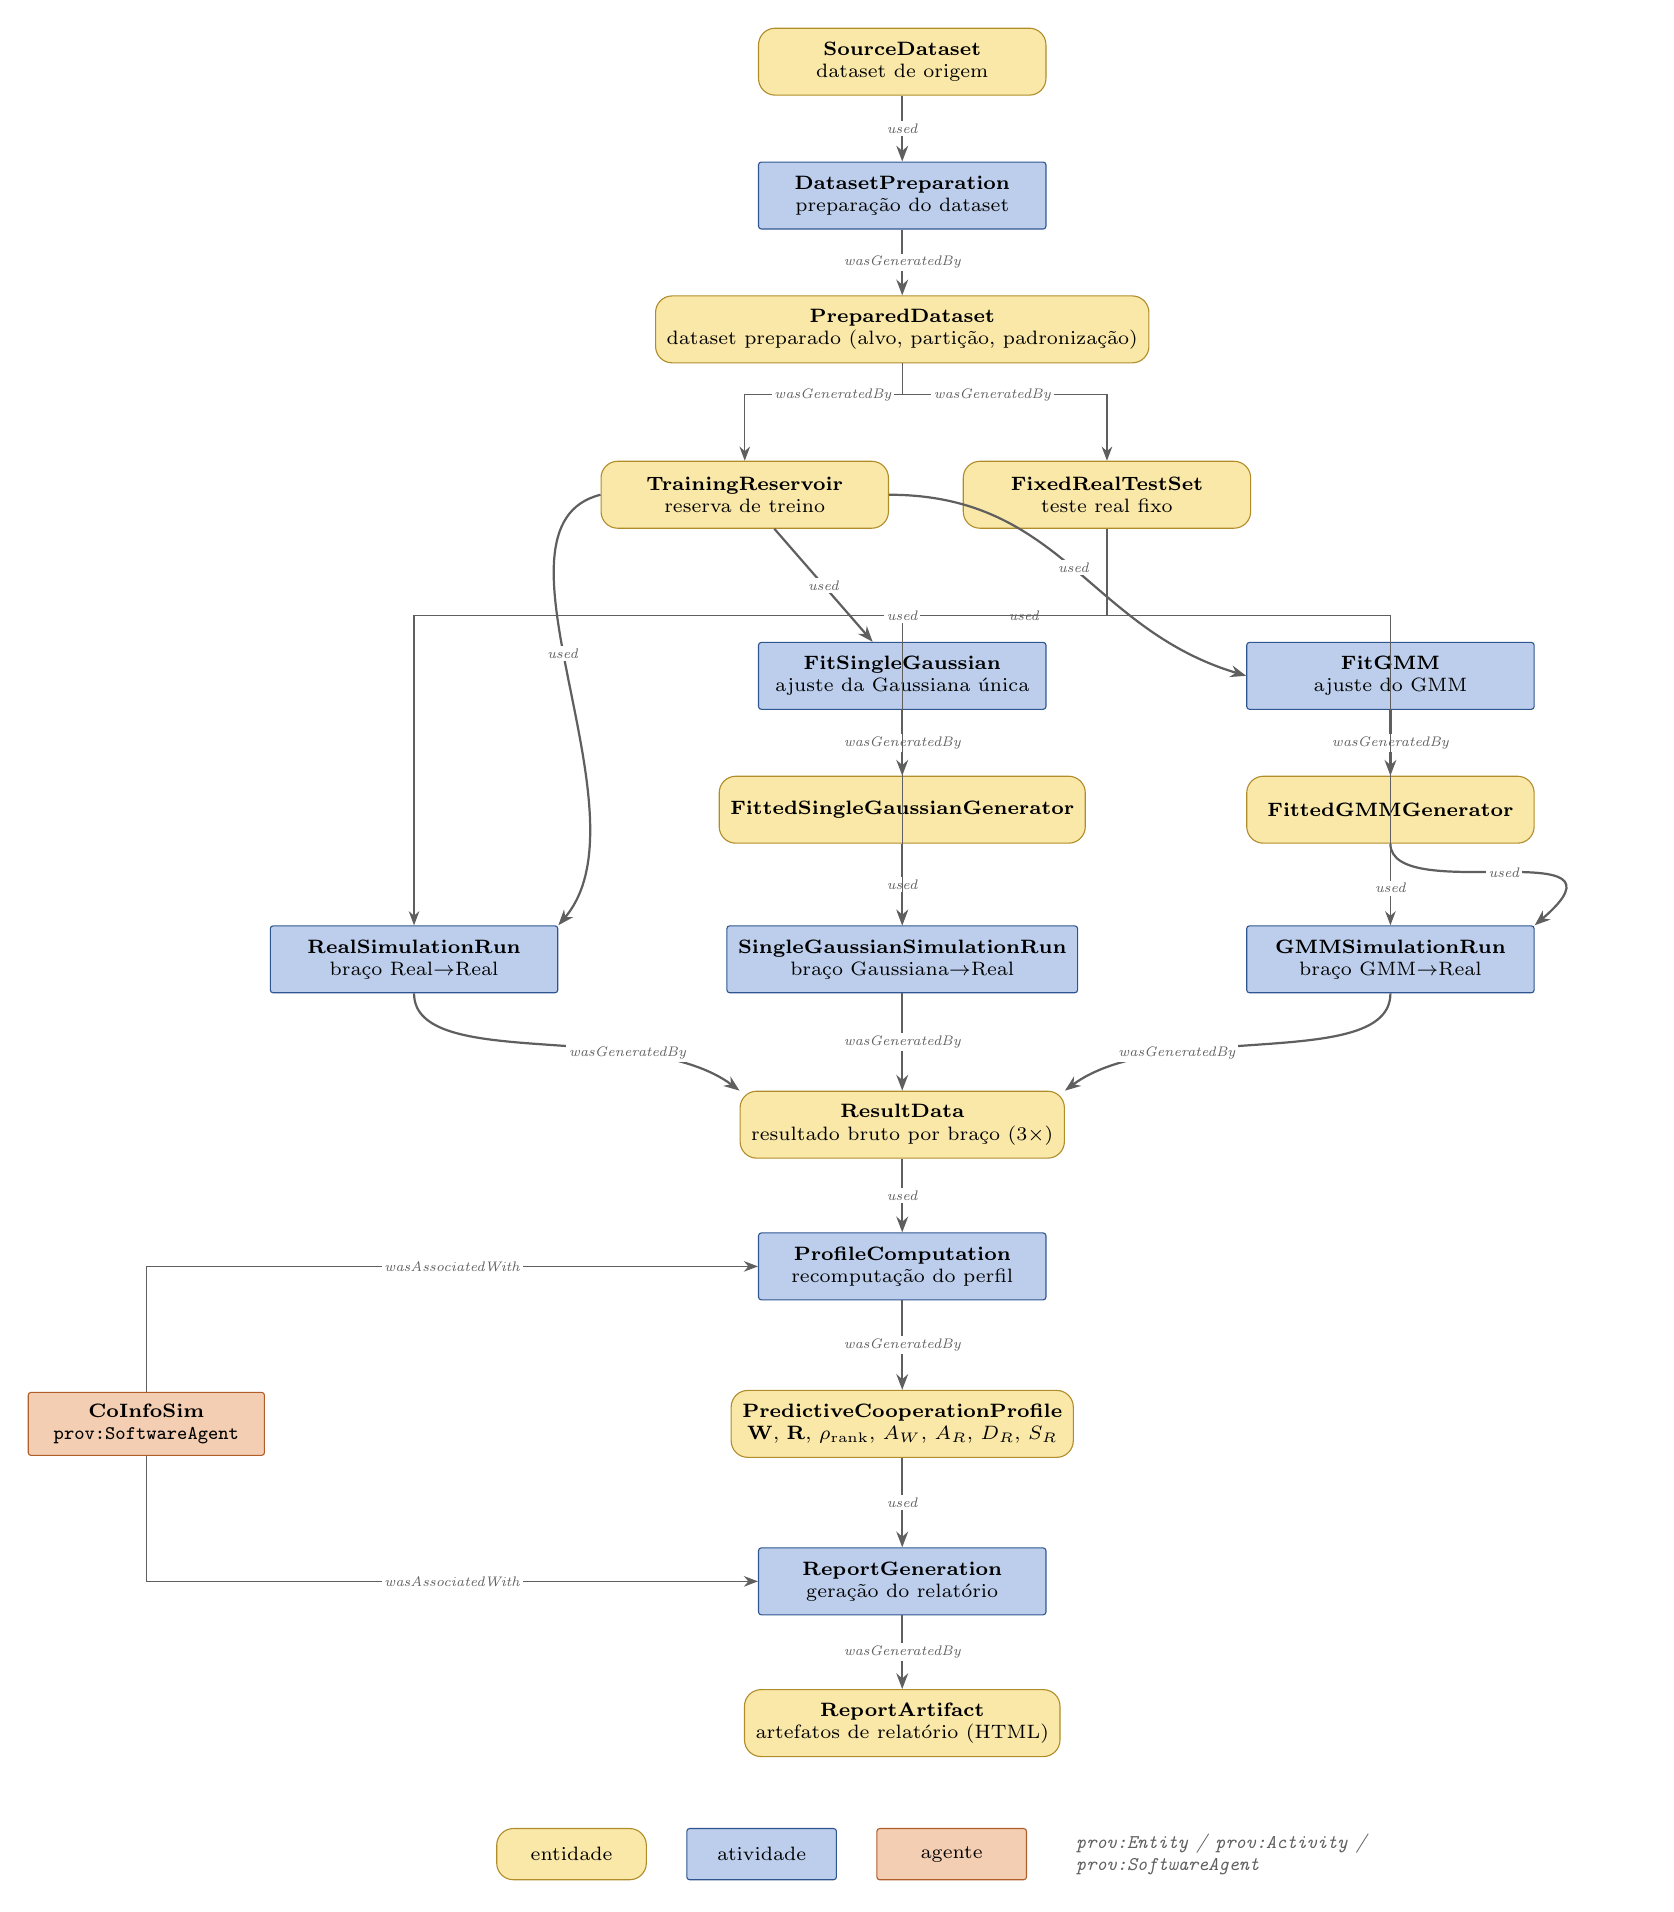
\begin{tikzpicture}[node distance=5mm and 5mm]

  % --- Preparação do dataset (tronco central) --------------------------------
  \node[entidade]  (source)   at (0, 20.4) {\textbf{SourceDataset}\\dataset de origem};
  \node[atividade] (dataprep) at (0, 18.7) {\textbf{DatasetPreparation}\\preparação do dataset};
  \node[entidade]  (prepared) at (0, 17.0) {\textbf{PreparedDataset}\\dataset preparado (alvo, partição, padronização)};

  % --- Partição treino/teste ---------------------------------------------------
  \node[entidade] (trainres) at (-2.0, 14.9) {\textbf{TrainingReservoir}\\reserva de treino};
  \node[entidade] (fixedtest) at (2.6, 14.9) {\textbf{FixedRealTestSet}\\teste real fixo};

  % --- Ajuste dos geradores (só a partir da reserva de treino) ----------------
  \node[atividade] (fitgauss)  at (0, 12.6) {\textbf{FitSingleGaussian}\\ajuste da Gaussiana única};
  \node[entidade]  (fittedgauss) at (0, 10.9) {\textbf{FittedSingleGaussianGenerator}};

  \node[atividade] (fitgmm)  at (6.2, 12.6) {\textbf{FitGMM}\\ajuste do GMM};
  \node[entidade]  (fittedgmm) at (6.2, 10.9) {\textbf{FittedGMMGenerator}};

  % --- Três braços de simulação (mesmo teste real fixo) -----------------------
  \node[atividade] (realrun) at (-6.2, 9.0) {\textbf{RealSimulationRun}\\braço Real$\to$Real};
  \node[atividade] (gaussrun) at (0, 9.0) {\textbf{SingleGaussianSimulationRun}\\braço Gaussiana$\to$Real};
  \node[atividade] (gmmrun) at (6.2, 9.0) {\textbf{GMMSimulationRun}\\braço GMM$\to$Real};

  % --- Resultado, perfil, relatório (tronco central) --------------------------
  \node[entidade]  (resultdata) at (0, 6.9) {\textbf{ResultData}\\resultado bruto por braço (3$\times$)};
  \node[atividade] (profcomp)   at (0, 5.1) {\textbf{ProfileComputation}\\recomputação do perfil};
  \node[entidade]  (profile)    at (0, 3.1) {\textbf{PredictiveCooperationProfile}\\$\mathbf{W}$, $\mathbf{R}$, $\rho_{\mathrm{rank}}$, $A_W$, $A_R$, $D_R$, $S_R$};
  \node[atividade] (reportgen)  at (0, 1.1) {\textbf{ReportGeneration}\\geração do relatório};
  \node[entidade]  (report)     at (0, -0.7) {\textbf{ReportArtifact}\\artefatos de relatório (HTML)};

  % --- Agente de software (associado às duas atividades de derivação) --------
  \node[agente] (agent) at (-9.6, 3.1) {\textbf{CoInfoSim}\\\texttt{prov:SoftwareAgent}};

  % --- Relações: preparação do dataset ---------------------------------------
  \draw[relacao] (source)   -- node[rlabel]{used} (dataprep);
  \draw[relacao] (dataprep) -- node[rlabel]{wasGeneratedBy} (prepared);
  \draw[relacaofina] (prepared.south) -- ++(0,-4mm) -| node[pos=0.22,rlabel]{wasGeneratedBy} (trainres.north);
  \draw[relacaofina] (prepared.south) -- ++(0,-4mm) -| node[pos=0.22,rlabel]{wasGeneratedBy} (fixedtest.north);

  % --- Relações: ajuste dos geradores (somente reserva de treino) ------------
  \draw[relacao] (trainres) -- node[rlabel]{used} (fitgauss);
  \draw[relacao] (fitgauss) -- node[rlabel]{wasGeneratedBy} (fittedgauss);
  \draw[relacao] (trainres.east) .. controls +(2.2,0) and +(-2.0,0.6) .. node[rlabel,pos=0.5]{used} (fitgmm.west);
  \draw[relacao] (fitgmm) -- node[rlabel]{wasGeneratedBy} (fittedgmm);

  % --- Relações: três braços de simulação -------------------------------------
  \draw[relacao] (trainres.west) .. controls +(-1.6,-0.4) and +(1.2,1.4) .. node[rlabel,pos=0.45]{used} (realrun.north east);
  \draw[relacao] (fittedgauss) -- node[rlabel]{used} (gaussrun);
  \draw[relacao] (fittedgmm.south) .. controls +(0,-0.8) and +(1.4,1.2) .. node[rlabel,pos=0.5]{used} (gmmrun.north east);

  % teste real fixo usado pelos três braços (mesma entidade)
  \draw[relacaofina] (fixedtest.south) -- ++(0,-1.1) -| node[pos=0.06,rlabel]{used} (realrun.north);
  \draw[relacaofina] (fixedtest.south) -- ++(0,-1.1) -| node[pos=0.5,rlabel]{used} (gaussrun.north);
  \draw[relacaofina] (fixedtest.south) -- ++(0,-1.1) -| node[pos=0.94,rlabel]{used} (gmmrun.north);

  % --- Relações: resultado, perfil, relatório ---------------------------------
  \draw[relacao] (realrun.south)  .. controls +(0,-1.0) and +(-1.2,0.9) .. node[rlabel,pos=0.7]{wasGeneratedBy} (resultdata.north west);
  \draw[relacao] (gaussrun)       -- node[rlabel]{wasGeneratedBy} (resultdata);
  \draw[relacao] (gmmrun.south)   .. controls +(0,-1.0) and +(1.2,0.9) .. node[rlabel,pos=0.7]{wasGeneratedBy} (resultdata.north east);
  \draw[relacao] (resultdata) -- node[rlabel]{used} (profcomp);
  \draw[relacao] (profcomp)   -- node[rlabel]{wasGeneratedBy} (profile);
  \draw[relacao] (profile)    -- node[rlabel]{used} (reportgen);
  \draw[relacao] (reportgen)  -- node[rlabel]{wasGeneratedBy} (report);

  % --- Agente -> as duas atividades de derivação do artefato final -----------
  \draw[relacaofina] (agent.north) |- node[pos=0.75,rlabel]{wasAssociatedWith} (profcomp.west);
  \draw[relacaofina] (agent.south) |- node[pos=0.75,rlabel]{wasAssociatedWith} (reportgen.west);

  % --- Legenda ------------------------------------------------------------
  \node[entidade, minimum width=1.9cm, minimum height=6.5mm, below=9mm of report, xshift=-4.2cm] (legent) {entidade};
  \node[atividade, minimum width=1.9cm, minimum height=6.5mm, right=5mm of legent] (legact) {atividade};
  \node[agente, minimum width=1.9cm, minimum height=6.5mm, right=5mm of legact] (legag) {agente};
  \node[rotulo, right=5mm of legag, align=left, text width=5.6cm, font=\scriptsize\itshape] {\texttt{prov:Entity} / \texttt{prov:Activity} /\\\texttt{prov:SoftwareAgent}};

\end{tikzpicture}
\end{document}
